\documentclass{article}

\usepackage{tikz}
\usetikzlibrary{arrows,calc}
\begin{document}
%
\section{Quad 2D}
\begin{itemize}
    \item Number of nodes in a row: $n$
    \item Total number of nodes: $n^2$
    \item Number of elements in a row: $n-1$
    \item Total number of elements:: $(n-1)^2$
    \item Node 0 is in the bottom left corner of the domain (element 0 is also in the bottom left corner).
    \item Increasing node number increases column index first, then row index.
\end{itemize}
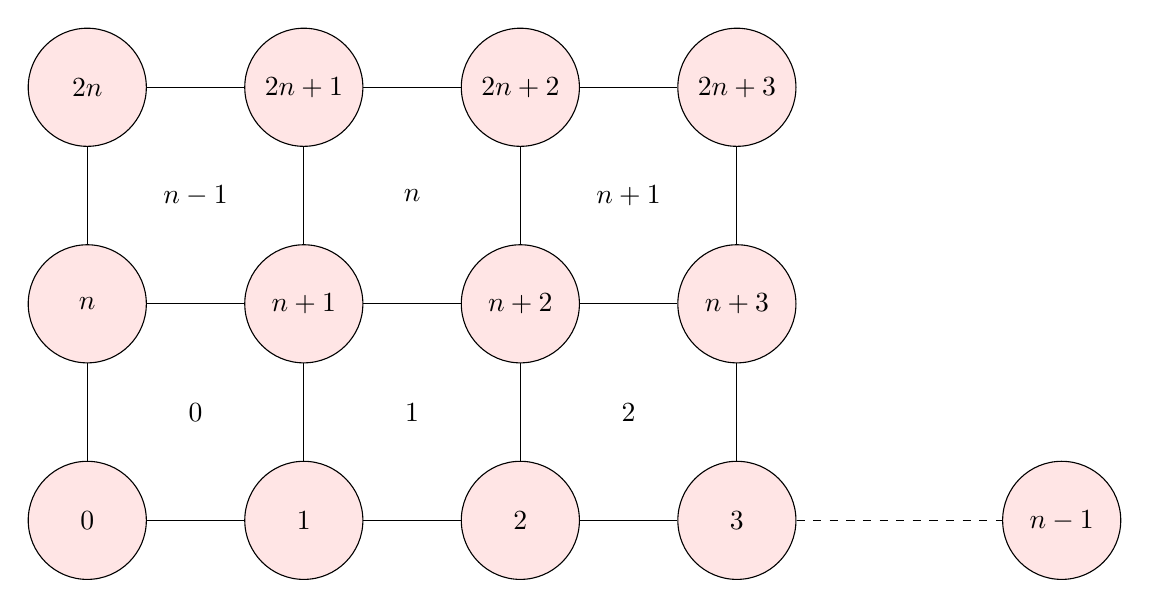
\begin{tikzpicture}[auto,>=latex']
    \tikzstyle{n}=[circle, draw=black, minimum size=1.5cm, fill=red!10]
    \coordinate (xdiff) at (2.75cm, 0);
    \coordinate (ydiff) at (0, 2.75cm);
    \node[n] (N0) at (0,0) {$0$};
    \node[n] (N1) at ($(xdiff) + (N0)$) {$1$};
    \node[n] (N2) at ($(xdiff) + (N1)$) {$2$};
    \node[n] (N3) at ($(xdiff) + (N2)$) {$3$};
    \node[n] (Ne) at ($1.5*(xdiff) + (N3)$) {$n-1$};
    \node[n] (N01) at ($(ydiff) + (N0)$) {$n$};
    \node[n] (N11) at ($(ydiff) + (N1)$) {$n+1$};
    \node[n] (N21) at ($(ydiff) + (N2)$) {$n+2$};
    \node[n] (N31) at ($(ydiff) + (N3)$) {$n+3$};
    \node[n] (N02) at ($(ydiff) + (N01)$) {$2n$};
    \node[n] (N12) at ($(ydiff) + (N11)$) {$2n+1$};
    \node[n] (N22) at ($(ydiff) + (N21)$) {$2n+2$};
    \node[n] (N32) at ($(ydiff) + (N31)$) {$2n+3$};
    \draw (N0) -- (N1) -- (N2) -- (N3);
    \draw (N01) -- (N11) -- (N21) -- (N31);
    \draw (N02) -- (N12) -- (N22) -- (N32);
    \draw (N0) -- (N01) -- (N02);
    \draw (N1) -- (N11) -- (N12);
    \draw (N2) -- (N21) -- (N22);
    \draw (N3) -- (N31) -- (N32);
    \draw[dashed=on] (N3) -- (Ne);
    \node at ($0.5*(N0) + 0.5*(N11)$) {$0$};
    \node at ($0.5*(N1) + 0.5*(N21)$) {$1$};
    \node at ($0.5*(N2) + 0.5*(N31)$) {$2$};
    \node at ($0.5*(N01) + 0.5*(N12)$) {$n-1$};
    \node at ($0.5*(N11) + 0.5*(N22)$) {$n$};
    \node at ($0.5*(N21) + 0.5*(N32)$) {$n+1$};
\end{tikzpicture}

\section{Tri 2d}

\end{document}
